%!TEX root = ../crimson_throne_book_main.tex
% 2014-12-31
Travelling through Korvosa's sewers brings back memories of the days when Sjo, Balian and Quint were still in Lamm's lambs and had to hunt for rats to feed Lamm's ever-hungry alligator Gobblegut. Only this time they are here to make peace with the rats instead of kill them. With Meep Gildenglare's pet rat Mr. Nibbles leading the way through this filthy maze the companions make good time. Even an ochre jelly that drops from the ceiling hardly slows them down. While Balian hacks the slime into ever smaller parts, Sjo finishes them off with a few {\itshape burning hands} spells. When they approach the wererats' den they notice some light seeping from a man-sized crack that cuts deep across the opposite wall of the tunnel, on the other side of the muck. Balian also picks up some voices from within. The companions decide to go the diplomatic way once again and hail the inhabitants of this underground lair with loud hellos. They continue calling out for Girrigz, the wererat leader,\hyperref[fig:Korvosa-entrance-to-wererat-den-503383346]{ as they approach the cleft } . Balian is the first to enter a rough-hewn stone cave, wading in the small flow of sewers filth that cuts through this room. An empty table bathes in the light of a flickering brazier. The perceptive ranger spots a shadow in the far end of the room, a shape that looks like a big, walking rat. With a squeaking voice it wonders what the companions want. \\

\begin{figure}[h]
	\centering
	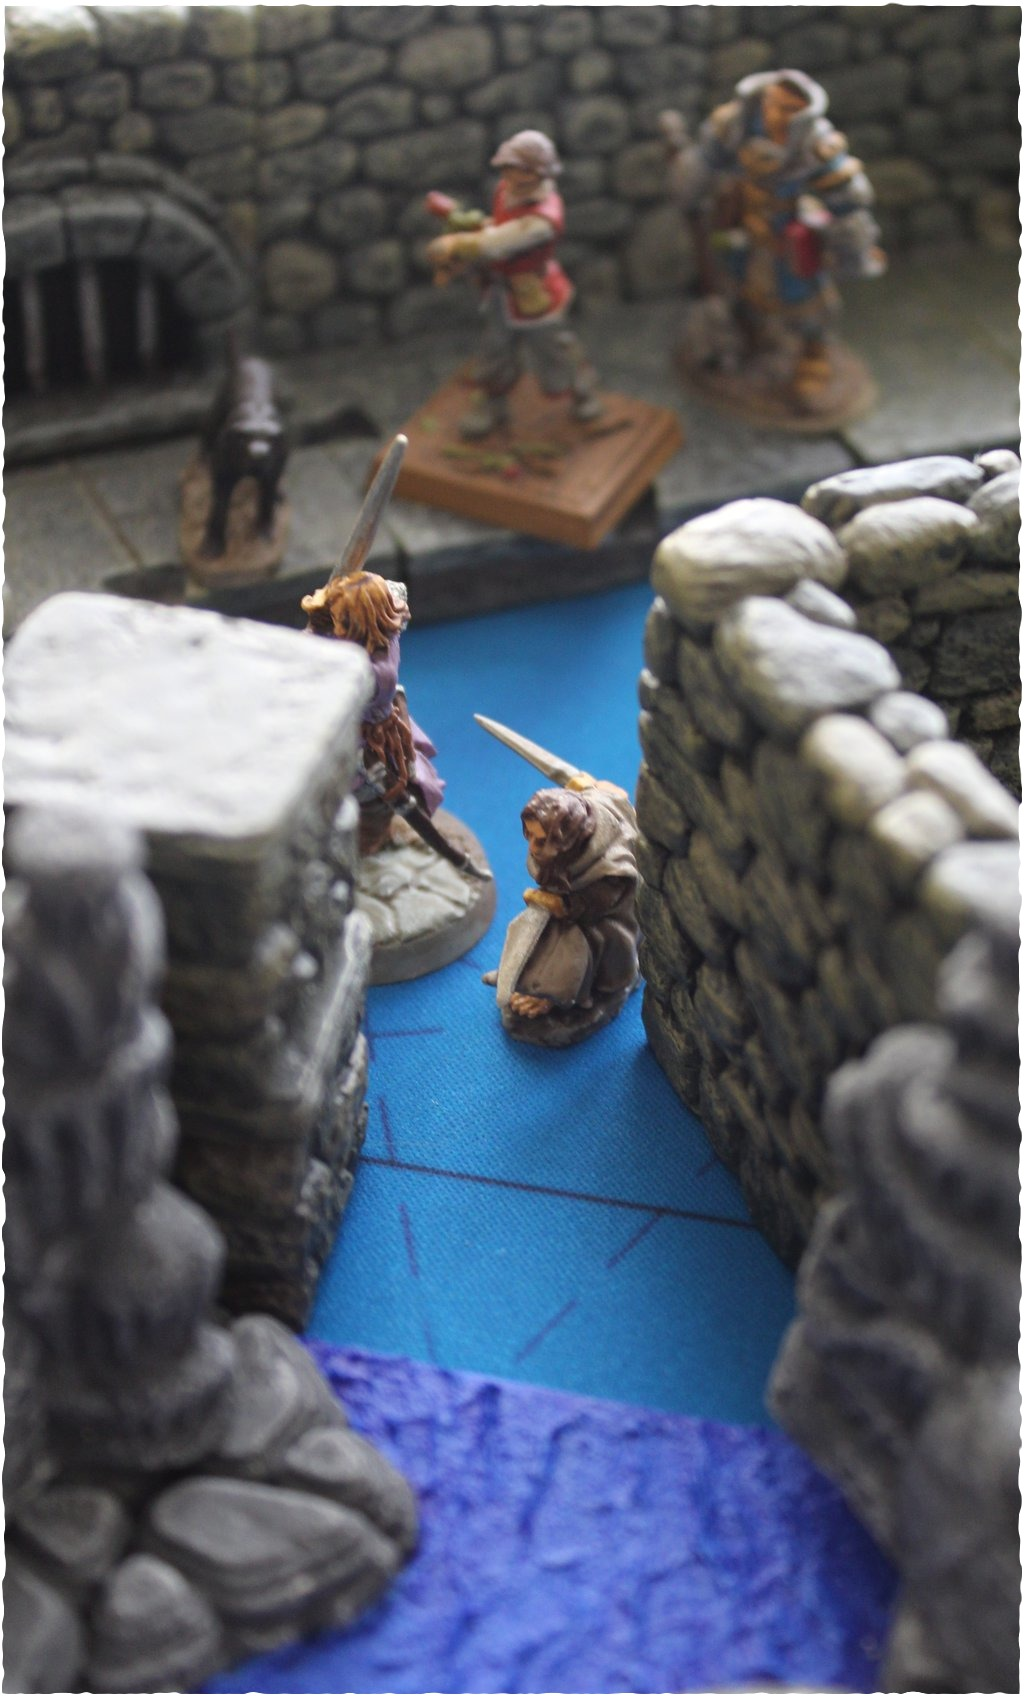
\includegraphics[width=0.4\textwidth]{images/Korvosa-entrance-to-wererat-den-503383346_mod.jpg}
	\caption{Korvosa entrance to wererat den}
	\label{fig:Korvosa-entrance-to-wererat-den-503383346}
\end{figure}

"We are here to talk to Girrigz about the sick rats and people. A mutual friend asked us to check on you to make sure you are okay", Quint answers.\\

"What do you mean, sick people? My people, you mean? My people are sick, as are our rat brothers", the creature interjects.\\

"You don't know, then? The people in the city are sick as well, maybe one in four is infected by now, and many rats as well", Sjo replies. "Some citizens blame you and we just want ascertain ourselves of the fact that this hasn't gone down wrong with you?"\\

"Hmmrr, so the people blame us ... again, while they are the ones who are guilty! It's always the same with you people ...", a much lower-pitched voice grunts from an opening in the other end of the room.\\

"Are you Girrigz? Meep Gildenglare sent us", Quint inquires.\\

"Meep, har har, that old little turncoat human lover ... she has turned from her own, we have no interest in what she has to say",\hyperref[fig:Korvosa-wererat-den-Girrigz-503384054]{ Girrigz } groans back. "No, ignorant intruders, we are not responsible for this mess, on the contrary, it is all a vicious plan of your kind to decimate my folk. It is humans who set loose the diseased rats on the city, when they had that ship sink in the river bend." \\

\begin{figure}[h]
	\centering
	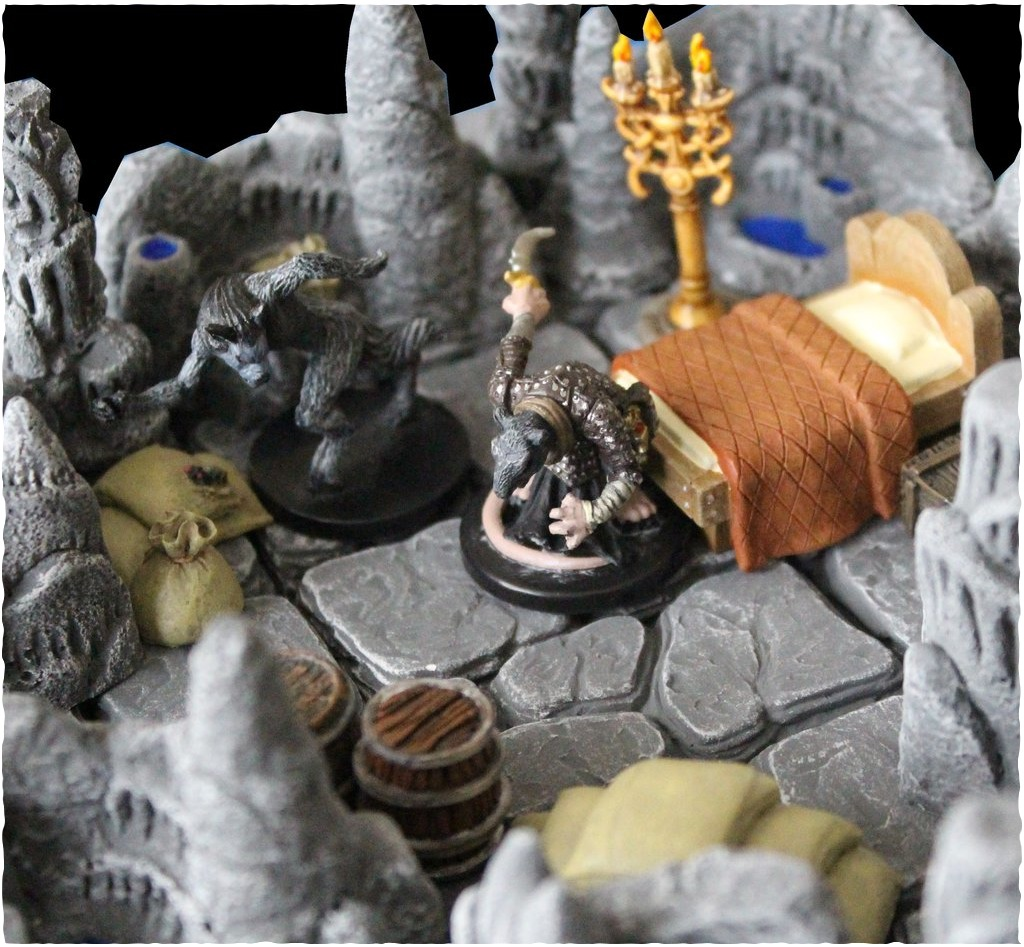
\includegraphics[width=0.4\textwidth]{images/Korvosa-wererat-den-Girrigz-503384054_mod.jpg}
	\caption{Korvosa wererat den Girrigz}
	\label{fig:Korvosa-wererat-den-Girrigz-503384054}
\end{figure}

Quint realizes that the wererat does not have a correct picture of the situation above ground. "Well, first of all, it is definitely not 'all the humans' who are responsible. Thousands are sick as well and hundreds have already lost their lives. I'm even infected myself. So your analysis that the humans are responsible is not accurate. But I do believe you when you say that some humans might be responsible. Sometimes there are bad people and if you can offer any insight on what happened, we'd be happy to learn about it."\\

"So humans are sick as well ... the irony, struck down by your own kind! But don't you have healers up there who can make the sickness go away?"\\

"We do, I am somewhat of a healer myself", Sjo returns. "But the plague has taken on huge proportions, so we are struggling to save just a few. Still, you have sick here as well? I can have a look at them if you want me to, although I do not master the magic to heal them."\\

"Well, maybe I do ... that is to say, I am in possession of a magical wand that is supposed to heal the sick, but I lack the power to activate it. Maybe you are capable of doing so?" Girrigz inquires with a friendlier voice. "I'll send one of my brothers to fetch you, follow him, but only you, big man, the rest of you will remain where they are."\\

The shifty ratman that Balian noticed before reappears in the north exit and waves Sjo closer. He leads the Shoanti through a smaller cave that reeks of death and decay. Hundreds of dead rats and at least seven deceased humanoids have been piled to the wall. The next room in the\hyperref[fig:Korvosa-wererat-sewer-dens-503381693]{ complex } is bigger, a small fire burns in the center and lights up the features of a dangerous-looking wererat, obviously Girrigz. Four very sick wererats are lying on the floor and more lycanthropes and dire rats move in the background. Quint sees that some of them shows signs of the plague as well. \\

\begin{figure}[h]
	\centering
	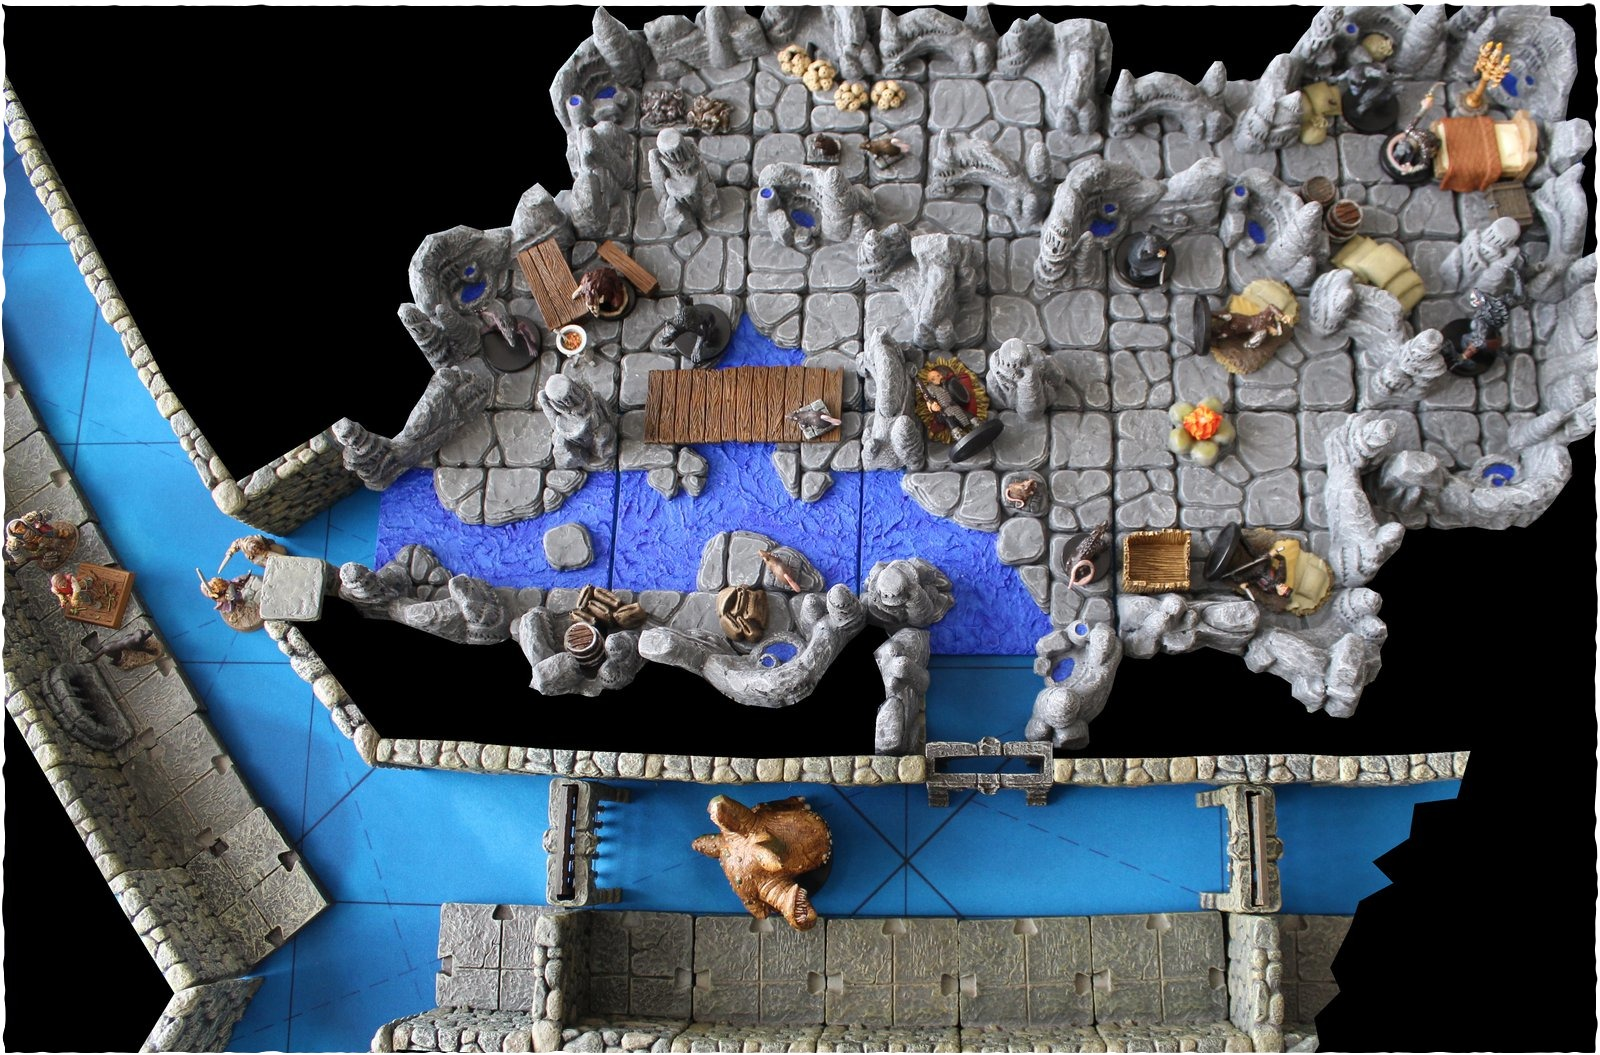
\includegraphics[width=0.4\textwidth]{images/Korvosa-wererat-sewer-dens-503381693_mod.jpg}
	\caption{Korvosa wererat sewer dens}
	\label{fig:Korvosa-wererat-sewer-dens-503381693}
\end{figure}

The healer examines one of the diseased creatures, he won't last another day if he receives no care. Girrigz comes closer and hands Sjo a white wand. "It should contain the magic to cure diseases." Sjo accepts the item and moves his other hand inside his pocket to reach for Zellara's deck. The fortuneteller's cards confirm that the wand does what Girrigz says. Of course, Sjo realizes, there is only a limited chance that the magic will have the desired effect. By his calculations that shouldn't even be one in two since wands are usually made at minimal caster level. Furthermore he does not know if the wererat is aware of that; so he tries to formulate it in a simpler fashion: "Your men are in bad shape, I'm afraid. I hope they are not too far gone to be cured. There, let me try it on this poor man first." Sjo activates the magic and the wererat immediately lets out a sigh of relief as his sores disappear and a healthy blush returns to his cheeks. So fortune favored the Shoanti on this first patient, but there still are three more badly diseased lycanthropes in the room. Sjo's attempts to cure these creatures meet with less success, as only one of them gets better. Sjo even retries healing the last one with a second charge, but that fails as well. "I'm afraid your brothers are too far gone", he whispers, knowing all too well that failure has nothing to do with the patient's condition, but with the strength of the wand. When Girrigz seems to accept this fact, the Shoanti is relieved, but he quickly fears that his little bluff might be pierced when Girrigz asks him to cure three other less sick wererats. Still, fortune favors the Shoanti once again as all three attempts to cure these three succeed on the first try. So his story holds.\\

Girrigz is now fully convinced of the companions' good intentions and invites all of them into the room to negotiate. When Sjo tells him that the magically cured are not immune to the disease and might get infected again, the wererat leader nods and suggests that it might not be a bad idea to lead the sick rats out of the city. The fierce lycanthrope looks nothing like the pied piper from the fairy-tale, but he might have the same sway over rodents and taking the infected rats out of the city would be a giant leap in fighting the plague.\\

Girrigz also confirms what the companions suspected already. The mysterious plague is connected to the ship that sunk in the harbor over a week ago. The wererat was alerted to the burning vessel by one of his rat friends. He went to the exit of the east tunnel to witness the ship go down, as hundreds of rats fled from the wreck. "It is customary for a boat to hold a few dozen rats, but this ship had far too many of them, many hundreds, some of whom swam to my location. That was the first time I saw the festering sores that have since then taken out half my crew. Strangely enough, there were no human survivors trying to reach the shore."\\

The companions decide that the wreck deserves closer inspection. Still, they were sent here with a mission as well, making sure that Girrigz does not take out his ire on the humans above. Sjo steers the conversation in this direction again, but first he wants to improve his goodwill and digs out the {\itshape restorative ointment} from his pack, knowing that this salve has the same chance to cure the sick as the wand did. "I might have one more trick up my sleeve to help your sick friends", he says. He applies some of the ointment on the last two sick wererats and as if by a miracle, they both work! Girrigz is very interested in the unguent and proposes to trade it for the wand. Sjo immediately sees the gain in this deal and accepts: there are only two applications of ointment left, while the wand still holds twenty charges. On the other hand, the wererat leader has no use for a wand he cannot activate, so it is a win-win situation. When the companions ask Girrigz not to seek revenge on the humans, he quickly agrees. The thought had crossed his mind, but the information and the aid the party provided him and his people sufficed to sway him. The company parts in good spirits. That evening Sjo uses the wand to cure the children in the villa and little Brienna. He also secures a sloop for tomorrow and arranges with Larella that she will forego one {\itshape cure disease} spell in favor of some  {\itshape water breathing} magic. 